% Formatting of listings
\lstset{language=C, frame=L, basicstyle=\footnotesize,%\sffamily,
	keywordstyle=\bfseries, showstringspaces=false, xleftmargin=\parindent, numbers=none, numberstyle=\tiny, stepnumber=2, numbersep=14pt}
\newpage
\section{Проектирование и тестирование}
\label{sec:Design}

\subsection{Требования к системе}
\label{sec:Requirements}
\textbf{Функциональные требования.}

Функциональные требования определяют действия, которые должна выполнять программа.

 \begin{itemizecustom}
 \item 
 
\fxnote{}
 \end{itemizecustom}

\textbf{Нефункциональные требования.}

Нефункциональные действия определяют свойства программы (удобство использования, безопасность и т.д.).

 \begin{itemizecustom}
 \item 
 
\fxnote{}
 \end{itemizecustom}

\subsection{Варианты использования системы}
\label{sec:Using}

Для проектирования приложения была построена модель взаимодействия пользователя с приложением в виде диаграммы вариантов использования. \fxnote{}

\subsection{Архитектура системы}
\label{sec:Architecture}

В данном разделе рассматривается архитектура приложения в виде диаграммы компонентов, которая показывает разбиение системы на структурные компоненты. Спроектированная архитектура приложения представлена на рисунке~\ref{ris:architecture} в виде диаграммы компонентов.

\begin{center}
    \begin{figure}[H]
        \center{\includegraphics[width=0.4\linewidth]{image}}
        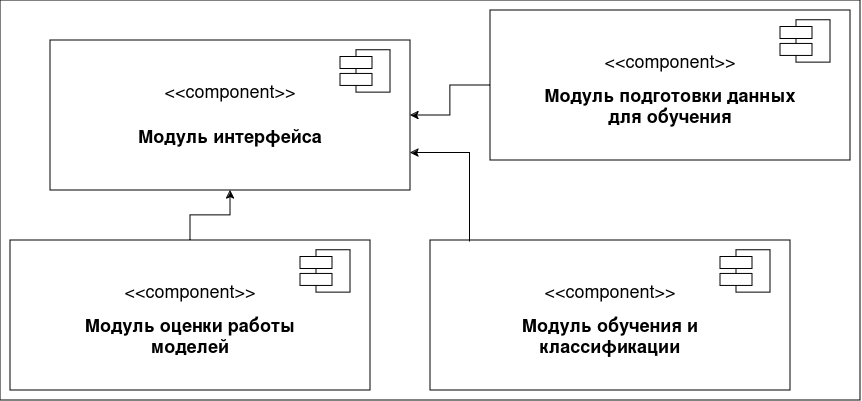
\includegraphics[scale=0.5]{pic/architecture.png}
        \caption{Архитектура системы}
        \label{ris:architecture}
    \end{figure}
\end{center}
\vspace{1.5em}

\textit{Модуль интерфейса} представляет собой главный (головной) модуль для отображения работы классификатора, с которым пользователь может взаимодействовать, и осуществляет работу остальных модулей.

\textit{Модуль оценки работы моделей} представляет собой набор алгоритмов, позволяющих оценить <<качество>> представленных способов определения класса популярности. В данном модуле используются такие метрики, как accuracy, precision, recall и F-score.

\textit{Модуль подготовки данных для обучения} используется для представления всех полей из датасета с целью последующей работы с ними. Данный модуль создает подробный датасет с полями <<forks>>, <<stars>>, <<pull-requests>> и другие.

\textit{Модуль обучения и классификации} представляет собой основной алгоритм программы. С помощью выбранной модели он определяет  класс популярности проекта на основе обучающей части датасета. Так, результатом является число популярности класса от 1 до 10.

\subsection{Графический интерфейс}
\label{sec:Graphical-interface}

В данном разделе будут представлены спроектированные макеты пользовательского интерфейса приложения. Данные макеты являются примерным представлением итогового продукта и содержат в себе основные необходимые функции.

Главная страница содержит в себе форму для отправки данных для определения класса популярности. Кроме того, окно содержит семь полей для данных по всем параметрам, включая имя репозитория и численных характеристики. А также выбор модели из выпадающего списка для определения класса популярности и кнопку, которая переадресует на другую страницу с результатами. На рисунке~\ref{ris:sketch} представлен макет формы ввода.

Страница c результатом определения класса популярности проекта содержит в себе форму с определенным классом в виде числа от 0 до 10. Та же информация, что была представлена для классификации, также представлена в качестве указания на то, что система верно интерпретировала данные.

 \fxnote{} 

\begin{center}
    \begin{figure}[H]
        \center{\includegraphics[width=0.6\linewidth]{image}}
        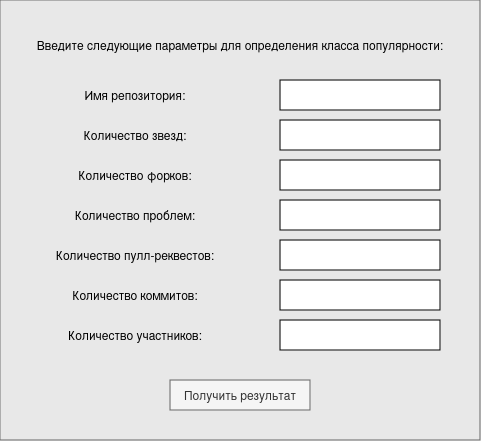
\includegraphics[scale=0.7]{pic/sketch-form.png}
        \caption{Макет формы для ввода}
        \label{ris:sketch}
    \end{figure}
\end{center}
\vspace{1.5em}